\section{I/O subsystem virtualisation and device mapping}
The input-output virtualisation process shows to be a challenging endevour due to the vast amount of pheripheral and the need to translate memory references used by Direct Memory Access (DMA) controllers \cite{smith2005virtual}.

Inside a guest virtual machine, all processes use translated logical or virtual addresses, however physical I/O devices, DMA controllers, and channel processes operates independently of the processor's Memory Management Unit (MMU) and require real physical addresses to peform direct data transfers into RAM \cite{goldberg1973architectural}.

Because disk controllers or network cards cannot dynamically traverse the guest's page tables during a bus transfer, the problem of address absolution arises as any more addresses stored by a guest program in the registers of a network or storage controller must be intercepted and converted into the host's real physical addresses by the hypervisor before the physical I/O hardware is put into operation \cite{goldberg1973architectural, smith2005virtual}.

\begin{figure*}[htbp]
    \centering
    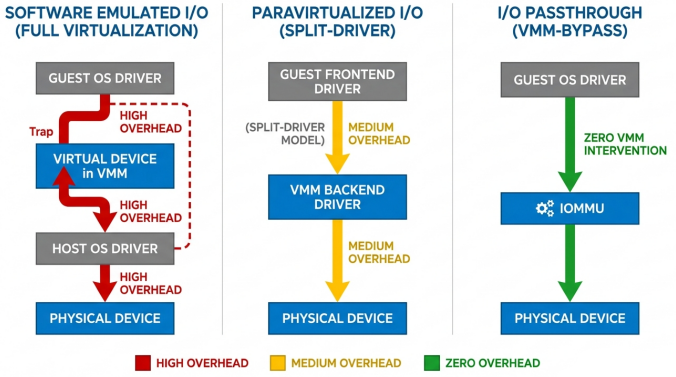
\includegraphics[width=0.8\linewidth]{images/diagrama-virtualizare-io.png}
    \caption{I/O virtualization paradigms and execution paths.}
    \label{fig:io-virtualisation-diagram}
\end{figure*}

The control and address translation flow proceeds as follows \cite{smith2005virtual}. When the Guest OS attempts to initiate an I/O operation, it executes a privileged Start I/O instruction. Because the Guest OS runs downgraded, Ring 1/3, the instruction generates a hardware trap in the hypervisor. The hypervisor takes control and accesses the channel program written by the guest. It sequentially traverses all CCW instructions and performs the 'absolutization' process: it translates each virtual buffer address from the CCW into absolute real physical addresses of the host using shadow page tables ($f \circ \phi$). To avoid Time-of-Check to Time-of-Use vulnerabilities, where the virtual machine could modify the addresses in the CCW during the execution of the hardware transfer, the hypervisor copies the entire CCW program into a private, protected memory area, Shadow CCW.


In historic systems that are based on channels, such as IBM VM/370, I/O operations were virtualised by running channel programs made of Channel Command Words (CCW) \cite{smith2005virtual}. Such process can be seen in the figure \ref{fig:io-virtualisation-diagram}.

\subsection{Types of interception interfaces}
The hypervisor can intercepent input-ouput operations at three distinct levels in the gust system's software stack \cite{smith2005virtual}.
    
    \begin{enumerate}
        \item Operation-Level Interface (Instruction level): Intercepts the processor's raw I/O instructions (\emph{IN, OUT, OUTS on x86}) or the memory mapped input-output writes to virtual device registers. It is an extremly slow method because each logical operation requires thousand of micro-instructions and each generates a VMExit trap.
        \item Device Driver Interface (Driver level): Intercepts calls at the device driver level. This approach is extremly efficient but requires advanced paravirtualisation which limits the portability of unmodified guest systems.
        \item System Call Interface (System call level): Intercepts generic calls like \emph{read()} or \emph{write()} at the boundary between the application and the guest kernel, which is often encountered in process virtual machines \cite{smith2005virtual}.
    \end{enumerate}

\subsection{I/O architecture on type II hypervisors}
In order to ensure compatibility with the high range of hardware available, type II hypervisors, such as VirtualBox and VMware, use a hybrid I/O architecture composed of three elements \cite{king.pdf}. The VMMonitor residing in ring 0 is a native kernel component that intercepts privileged input-ouput instructions and runs fast software simulators for standard devices. VMApp, which resides in ring 3, is a user application on the host system. If the VMMonitor intercepts a complex I/O such network access it transfers the request to the VMApp which in return uses the host's system standard calls to send tasks to the host OS's native drivers. Lastly the VMDriver is a driver installed in host kernel that provides the fast comunication channel and the rapid switch between VMMonitor and VMApp \cite{king.pdf}.

\subsection{I/O Passthrough}
Software mechanisms which are either emulated or paravirtualized always introduce a performance penalty due to multiple buffer copies and constants VMExits therefore I/O passthrough or VMM-Bypass is a technology that completly eliminates the hypervisor from the equation. The hypervisor directly maps the physical I/O ports or the MMIO address space of a real device on the host machine, for example an NVIDIA video card or a 10G network card, into the guest virtual machine's physical address space. This native driver comunicates directly with the card's physical registers which in hence allows it to transmit data at native speeds with a very low performance overhead \cite{implementation-of-internetworking-with-host-internet-in-oracle-virtualbox-guest-virtual-machines.pdf}.

\subsection{IOMMU hardware technology}
While using I/O passthrough for things like virtual and network cards offers considerable benefits it also introduces a critical security risk and stability problem. How could a physical hardware device controlled by a guest system running in unprivileged mode write data via DMA into the host's real physical memory without corupting the hypervisor or other virtual machines? In order to solve this problem manufactures introduced a new physical component named IOMMU or Input-Ouput Memory Management Unit or comercially known as Intel VT-d or AMD-Vi \cite{vm-security.pdf}. Thus the IOMMU functions as a dedicated MMU for peripherals. The Input-Ouput Memory Management Unit mantains an I/O address translation page table in its hardware. When for example a netword card assigned to a virtual machine tries to execute a DMA write to the guest physical address provided by a guest driver the IOMMU intercepts the transaction directly on the PCIe bus and instantly translates it into the host's real physical address. Also the IOMMU instantly blocks any attempt by a hardware device to access via DMA RAM areas that were not explecitly mapped by the hypervisor to the virtual machine. If a compromised virtual machine attempts to use the host hardware to write into the hypervisor's kernel memory the IOMMU stops the transaction at the electricity level and flags a \emph{IOMMU Fault interrupt} thus preventing hardware based VM escape attacks \cite{vm-security.pdf}.